\documentclass[12pt,spanish,oneside]{book}
\usepackage{lmodern}
\usepackage{amssymb,amsmath}
\usepackage{ifxetex,ifluatex}
\usepackage{fixltx2e} % provides \textsubscript
\ifnum 0\ifxetex 1\fi\ifluatex 1\fi=0 % if pdftex
  \usepackage[T1]{fontenc}
  \usepackage[utf8]{inputenc}
\else % if luatex or xelatex
  \ifxetex
    \usepackage{mathspec}
  \else
    \usepackage{fontspec}
  \fi
  \defaultfontfeatures{Ligatures=TeX,Scale=MatchLowercase}
\fi
% use upquote if available, for straight quotes in verbatim environments
\IfFileExists{upquote.sty}{\usepackage{upquote}}{}
% use microtype if available
\IfFileExists{microtype.sty}{%
\usepackage{microtype}
\UseMicrotypeSet[protrusion]{basicmath} % disable protrusion for tt fonts
}{}
\usepackage[inner = 3cm, outer = 2cm, top = 2.5cm, bottom = 2.5cm]{geometry}
\usepackage{hyperref}
\hypersetup{unicode=true,
            pdftitle={Tesis de Licenciatura},
            pdfauthor={Paola Corrales},
            pdfborder={0 0 0},
            breaklinks=true}
\urlstyle{same}  % don't use monospace font for urls
\ifnum 0\ifxetex 1\fi\ifluatex 1\fi=0 % if pdftex
  \usepackage[shorthands=off,main=spanish]{babel}
\else
  \usepackage{polyglossia}
  \setmainlanguage[]{spanish}
\fi
\usepackage{longtable,booktabs}
\usepackage{graphicx,grffile}
\makeatletter
\def\maxwidth{\ifdim\Gin@nat@width>\linewidth\linewidth\else\Gin@nat@width\fi}
\def\maxheight{\ifdim\Gin@nat@height>\textheight\textheight\else\Gin@nat@height\fi}
\makeatother
% Scale images if necessary, so that they will not overflow the page
% margins by default, and it is still possible to overwrite the defaults
% using explicit options in \includegraphics[width, height, ...]{}
\setkeys{Gin}{width=\maxwidth,height=\maxheight,keepaspectratio}
\IfFileExists{parskip.sty}{%
\usepackage{parskip}
}{% else
\setlength{\parindent}{0pt}
\setlength{\parskip}{6pt plus 2pt minus 1pt}
}
\setlength{\emergencystretch}{3em}  % prevent overfull lines
\providecommand{\tightlist}{%
  \setlength{\itemsep}{0pt}\setlength{\parskip}{0pt}}
\setcounter{secnumdepth}{5}
% Redefines (sub)paragraphs to behave more like sections
\ifx\paragraph\undefined\else
\let\oldparagraph\paragraph
\renewcommand{\paragraph}[1]{\oldparagraph{#1}\mbox{}}
\fi
\ifx\subparagraph\undefined\else
\let\oldsubparagraph\subparagraph
\renewcommand{\subparagraph}[1]{\oldsubparagraph{#1}\mbox{}}
\fi

%%% Use protect on footnotes to avoid problems with footnotes in titles
\let\rmarkdownfootnote\footnote%
\def\footnote{\protect\rmarkdownfootnote}

%%% Change title format to be more compact
\usepackage{titling}

% Create subtitle command for use in maketitle
\newcommand{\subtitle}[1]{
  \posttitle{
    \begin{center}\large#1\end{center}
    }
}

\setlength{\droptitle}{-2em}
  \title{Tesis de Licenciatura}
  \pretitle{\vspace{\droptitle}\centering\huge}
  \posttitle{\par}
\subtitle{Desarrollo de una metodología de trabajo para caracterizar el ciclo
diurno del viento en la capa límite atmosférica a partir de datos de
radar meteorológico y su posterior uso para la validación de modelos.}
  \author{Paola Corrales}
  \preauthor{\centering\large\emph}
  \postauthor{\par}
  \date{}
  \predate{}\postdate{}

\linespread{1.25}
\usepackage{subfig}
\usepackage{hyperref}

\begin{document}
\maketitle

{
\setcounter{tocdepth}{3}
\tableofcontents
}
\renewcommand{\listtablename}{Índice de tablas} 
\renewcommand{\tablename}{Tabla} 

\listoffigures
\newpage

\listoftables
\newpage

\section*{Agradecimientos}\newpage

\section*{Resumen}\newpage

\chapter{Introducción}\label{introduccion}

La capa límite planetaria (CLP) corresponde a la porción de atmósfera
que se encuentra directamente influenciada por la superficie y que
responde a sus forzantes en una escala de tiempo de una hora o menos
(Stull, 1988). Los procesos que ocurren dentro de esta capa son de suma
importancia para entender y pronosticar la evolución de la atmósfera en
distintas escalas espaciales y temporales. En particular estos procesos
controlan el intercambio de energía entre la superficie y la atmósfera
afectando, entre otras cosas, las condiciones para la ocurrencia de
convección húmeda profunda y la intensidad de las circulaciones de
mesoescala, que tienen un alto impacto sobre las actividades humanas.

En nuestra región existen estudios que buscan caracterizar los procesos
que ocurren en la capa límite de forma tal de poder avanzar en su
entendimiento y su dependencia por ejemplo con las propiedades de la
superficie o el estado de la atmósfera (Mazzeo y Gassmann, 1990; Ulke,
2000; Gassmann y Mazzeo, 2001; Acevedo et~al., 2014; Tonti y Gassmann,
2015).

Dado que la ocurrencia de turbulencia en la capa límite planetaria se da
en múltiples escalas espaciales y temporales, la representación de los
procesos que ocurren dentro de ella es un desafío para los modelos
numéricos. Actualmene los modelos de simulación regional y global no
cuentan con la resolución necesaria para representar los procesos de la
CLP de forma explícita, debiendo recurrir a una representación
simplificada. De esta manera se simula numéricamente una parte del
espectro turbulento, mientras que los procesos en la escala de subgrilla
se resuelven a través de parametrizaciones con cierres de distinto
orden, es decir, con diferentes niveles de aproximaciones.

Existen diferentes alternativas para parametrizar los procesos de capa
límite pero pueden clasificarse en dos grandes grupos. De acuerdo a
Stull (1988), las parametrizaciones con clausura local determinan el
valor de cualquier variable desconocida en cada punto a partir del valor
o el gradiente de una variable conocida en el mismo punto; suponiendo
que la turbulencia tiene un comportamiento análogo a la difusión
molecular. Por otro lado las parametrizaciones con clausura no local
asumen que la turbulencia está caracterizada por la superposición de
torbellinos de distintas escalas que transportan las características del
medio; y para lograr esto, el valor de la variable desconocida en un
punto es aproximada a partir de una variable conocida en varios puntos
en el espacio.

La validación de las parametrizaciones de CLP en distintas situaciones
sinópticas es un tema de gran interés debido a la necesidad de modelar
los procesos de subgrilla presentes que afectan procesos en el resto de
las escalas de variabilidad atmosférica (Xie et~al., 2012; Banks et~al.,
2016).

A nivel regional, la representación de la capa límite en los modelos
numéricos ha recibido mucha atención en las zonas oceánicas
(particularmente en los océanos tropicales, Wang et~al. (2004)). Sin
embargo, existen pocos estudios acerca del desempeño de las
parametrizaciones de capa límite en las regiones continentales (Ulke y
Andrade, 2001; Ruiz et~al., 2010; Berri et~al., 2012; Rizza et~al.,
2013).

Uno de los principales desafíos a la hora de estudiar los procesos que
ocurren en la capa límite o para validar cómo los modelos representan
dichos procesos, es la disponibilidad de observaciones. Las redes de
radiosondeos que permiten obtener perfiles de viento, temperatura y
humedad en la capa límite miden con frecuencias temporales de entre 12 y
24 horas (solo eventualmente cada 6 horas) lo que impide analizar la
evolución de las características de la CLP a lo largo del día.

Sin embargo los radares Doppler permiten estimar la componente radial
del viento en un radio horizontal de hasta 240 km y a partir de esa
información permiten reconstruir perfiles verticales de viento
utilizando la técnica Velocity Azimuth Display (VAD).

En días en los que no existen ecos producidos por hidrometeoros, los
radares pueden detectar la velocidad del viento dentro de la capa límite
a partir de blancos como los insectos, de acuerdo a Rennie et~al. (2010)
estos datos podrían ser utilizados si se elimina el efecto de los ecos
de terreno y otras observaciones erróneas. Las observaciones de radar
están disponibles con una frecuencia temporal de hasta 5 minutos
permitiendo obtener perfiles de viento con una resoloción temporal mucho
mayor.

La calidad de estos perfiles ha sido comparada con los perfiles
obtenidos a partir de radiosondeos, encontrándose en general que los
datos obtenidos resultan adecuados para su uso en el estudio de los
procesos de capa límite y en la verificación de modelos numéricos
(Bousquet et~al., 2008; Salonen et~al., 2008) y en la generación de
condiciones iniciales para pronósticos a muy corto plazo (Rennie et~al.,
2011).

Uno de los aspectos importantes a tener en cuenta en el uso de radares
para el estudio de los perfiles de viento, es la necesidad de aplicar un
riguroso control de calidad a los datos que permita solucionar diversos
aspectos que pueden afectar la confiabilidad de los mismo. Entre los
problemas más comunes se cuentan: contaminación por ecos de terreno,
efecto de aliasing, y contaminación por blancos móviles. Estos aspectos
deben ser abordados antes de poder utilizar los datos para estimar el
perfil de velocidad (Holleman et~al., 2008; Rennie et~al., 2011)
aplicando algoritmos de control de calidad (Rennie et~al., 2011; Ruiz
et~al., 2015).

La disponibilidad de la información de radar Doppler en Argentina ofrece
un gran recurso de información para estudiar las propiedades de la capa
límite planetaria en nuestra región y para validar la calidad de los
modelos numéricos a la hora de representar dichas propiedades.

El objetivo de esta Tesis de Licenciatura es desarrollar una metodología
para el estudio de los procesos de capa límite a partir de los datos de
radar y analizar el comportamiento de distintas parametrizaciones de CLP
disponibles en el modelo Weather Research and Forecasting (WRF -
Skamarock et~al. (2008)) al representar algunos de los procesos
presentes a lo largo del día.

Se plantea como hipótesis que los datos de viento radial obtenidos de
información de radar permiten estimar los perfiles verticales de viento
con una frecuencia temporal de 10 minutos, en un espesor que abarca
desde superficie y hasta 2000 m de altura, permitiendo realizar una
caracterización de la evolución temporal de dichos perfiles dentro de la
capa límite atmosférica. La estimación de esos perfiles permitirán
además validar las parametrizaciones de la capa límite que utilizan los
modelos numéricos con una mayor resolución temporal a la utilizada en
trabajos previos.

Para alcanzar el objetivo se realizó el siguiente procedimiento: En
primer lugar se determinaron las características necesarias para
identificar posibles casos de estudio que permitan analizar los procesos
de CLP asociados al ciclo diario. Luego se procesó los datos de radar
para caso en estudio y se aplicaron los controles de calidad necesarios
antes de realizar el cálculo del VAD desarrollado y validado como parte
de este trabajo. Se analizó la consistencia de los resultados obtenidos
y las características principales de la variación del viento a lo largo
del día. Para las simulaciones numéricas con el modelo WRF se define un
dominio y condiciones iniciales adecuadas para modelar un caso de
estudio utilizando algunas parametrizaciones disponibles. Se comparan
las simulaciones con las observaciones previamente obtenidas y se
analizan algunas variables asociadas a la turbulencia.

De esta manera, este trabajo permite desarrollar una metodología para el
tratamiento de observaciones no convencionales, su aplicación al estudio
de los procesos de CLP y al modelado numérico de los mismos.

\chapter{Metodología}\label{metodologia}

En esta sección se describen los datos utilizados en el trabajo y las
metodologías aplicadas al análisis.

\section{Región y casos de estudio}\label{region-y-casos-de-estudio}

Este trabajo centra el análisis en la región de la ciudad de Paraná
(provincia de Entre Ríos, Argentina) donde se encuentran el Radar
Doppler del INTA (Instituto Nacional de Tecnología Agropecuaria) y una
estación meteorológica de superficie perteneciente al SMN (Servicio
Meteorológico Nacional) separados por aproximadamente 9 kilómetros de
distancia.

\begin{figure}

{\centering 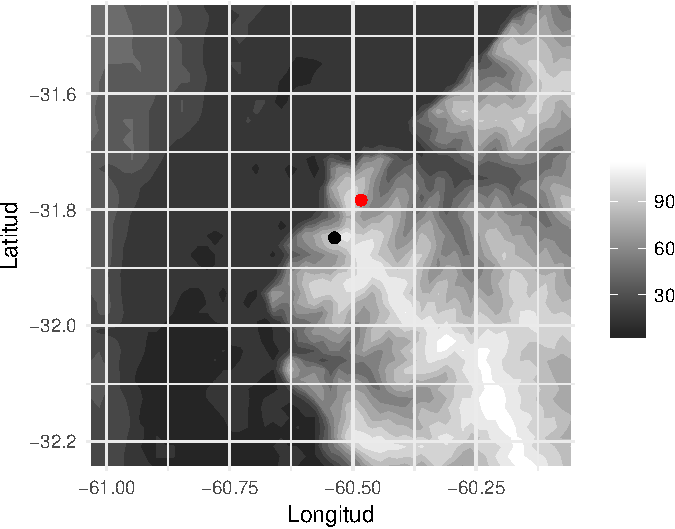
\includegraphics[width=0.75\textwidth]{Tesis_files/figure-latex/topografia-1} 

}

\caption[Topografía de la región en estudio en metros sobre el nivel del mar.]{Topografía de la región en estudio en metros sobre el nivel del mar. El punto negro indica la ubicación del Radar INTA Paraná, el punto rojo indica la ubicación de la estación Paraná Aero. \label{topografia}}\label{fig:topografia}
\end{figure}

La elevación de la región elegida muestra un mínimo de 5 metros sobre el
nivel del mar en la cuenca del Río Paraná y un máximo de aproximadamente
110 metros sobre el nivel del mar sobre el margen sudeste de río donde
ubica tanto la estación meteorológica como el radar (Figura
\ref{topografia}). La región está dominada por la presencia del río y
las regiones costeras donde predominan los campos de pastizales o pasto
con excepción la ciudad de Paraná (al norte), la ciudad de Santa Fé (al
noreste) y pequeños conglomerados de casas.

\subsection{Criterios utilizados para la selección de los casos de
estudio}\label{criterios-utilizados-para-la-seleccion-de-los-casos-de-estudio}

Con el objetivo analizar los procesos que ocurren en la CLP a lo largo
del día es necesario identificar aquellas condiciones atmosféricas que
permitan el desarrollo de la capa límite y al mismo tiene donde los
datos de radar sean confiables. Por lo tanto se buscaron cumplir los
siguientes criterios:

\begin{itemize}
\tightlist
\item
  \textbf{Viento moderado.} En estas situaciones los datos de radar son
  más confiables y permiten el desarrollo de la capa límite estable
  nocturna (Gassmann y Mazzeo, 2001).
\item
  \textbf{Cielos despejados.} Para garantizar el calentamiento desde la
  superficie y el desarrollo de una capa límite mezclada.
\item
  \textbf{Verano.} Donde el calentamiento es más intenso.
\end{itemize}

Las características previas se buscaron a partir del análisis de los
datos de la estación meteorológica de superficie Paraná Aero provistos
por el SMN y de reflectividad (dBZ) del radar de Paraná para los meses
de enero de 2016 y 2017.

En el primer tipo de datos se analizó la velocidad de viento, la
cobertura nubosa y la precipitación observada a cada hora. En el caso de
los datos de radar se observó la presencia de ecos meteorológicos en las
inmediaciones del radar (a una distancia menor a 150 km) en cada tiempo
disponible (aproximadamente cada 10 minutos). Un caso de estudio posible
será aquel que cumpla con las características mencionadas durante las 24
horas del día aunque es deseable que las condiciones se mantengan
durante las 12 horas previas al día en estudio ya que las
características de la capa estable nocturna puede ser influenciada por
las características de la capa mezclada del día anterior.

\subsection{Descripción de los casos de
estudio}\label{descripcion-de-los-casos-de-estudio}

A partir de análisis previamente descripto se identificaron 3 casos de
estudio que se describen a continuación.

\subsubsection{Caso 1: 14 de enero de
2016}\label{caso-1-14-de-enero-de-2016}

El caso 1 abarca el periodo de las 00 UTC del 14 de enero a las 00 UTC
del 15 de enero de 2016. A escala regional se observó un anticiclón
ubicado sobre el océano Atlántico y al este Uruguay a las 00 UTC de 14
de enero. Este sistema está asociado a vientos del noreste sobre el
dominio en estudio. En superficie se registraron vientos débiles
(menores a 2 m/s) del este y sureste en las primeras horas del periodo.
En la estación meteorológica se observó nubosidad alta en las primeras
horas de tipo cirroestrato que por momentos cortos cubrió el cielo. No
se observaron ecos meteorológicos en la región del radar. \textbf{Que
tanto afecta la nubosidad alta?}

Posteriormente, a las 12 UTC el anticiclón se intensifica y comienza a
moverse hacia el NE y en superficie se observan vientos predominantes
del noreste de hasta 6.5 m/s. No se observa nubosidad y la temperatura
en superficie alcanza los 32.4°C.

\textbf{Humedad relativa disminuye de 85\% a 35\% en el periodo, no me
queda clara la causa y tampoco se que tan importante puede ser esto
luego}

\subsubsection{Caso 2:}\label{caso-2}

\subsubsection{Caso 3:}\label{caso-3}

\section{Descripción de los datos de
radar}\label{descripcion-de-los-datos-de-radar}

El radar ubicado en Paraná (Provincia de Entre Ríos) emite energía
electromagnética en la banda C (4 a 8 GHz) y es de doble polarización.
La estrategia de escaneo de la atmósfera está programada para que la
antena de giros en sentido horizontal de 360º y cambie de elevación
sucesivamente 12 veces. El ángulo vertical varía entre 0.5° y 15.1°. El
rango del radar (distancia a la que llega la señal desde la ubicación
del radar) puede ser de 120, 240 y 480 km con una resolución espacial de
1 \(\mathrm{km^2}\) (Saibene et~al., 2014) de acuerdo a la estrategia de
escaneo.

El escaneo completo se realiza cada 10 minutos, dando 144 volúmenes de
datos diarios registrando para las distintas variables como
reflectividad (dBZ) y velocidad radial (\(V_r\)).

En este trabajo se usaron datos de radar con un rango de 240 km y 12
ángulos de elevación para los periodos comprendidos por cada caso de
estudios provistos por \textbf{XXXX INTA XXXX}

Cada volumen de dato correspondiente a un tiempo de escaneo completo fue
convertido al formato CfRadial con el paquete Radx C++ desarrollado por
Mike Dixon (NCAR - National Center for Atmospheric Research)
\textbf{CITA} para el posterior procesamiento y análisis. En particular
se utilizó la variable de reflectividad sin procesamiento para
determinar la presencia o no de ecos meteorológicos en el dominio
cercano al radar y la velocidad radial para la obtención de los perfiles
de viento.

\section{Tratamiento de aliasing}\label{tratamiento-de-aliasing}

Un problema importante al momento de utilizar los datos de velocidad
radial es la contaminación por aliasing ya que afecta significativamente
la calidad de los perfiles de viento finales, de acuerdo a Gao y
Droegemeier (2004) un 3\% de contaminación por aliasing puede generar un
error cuadrático medio del 50\% en el perfil de viento medio a partir de
la técnica VAD. El aliasing es la superposición de la señal de radar y
ocurre cuando la velocidad real supera a la velocidad de Nyquist
(\(V_N\)). Este parámetro es intrínseco a las características del radar
ya que depende de la frecuencia y estrategia de escaneo y en particular
de la frecuencia de repetición del pulso o señal que emite.

En el caso del radar de Paraná con la estrategia de escaneo de 240km de
rango, tiene una \(V_N = 6.7 m/s\) por lo que cualquier velocidad mayor
se verá afectada por el aliasing. Esto puede verse en la Figura
\ref{aliasing}, las regiones con aliasing se son aquellas que donde el
valor de la velocidad radial salta al extremo opuesto de la escala.

Existen muchos algoritmos que buscan solucionar el problema del aliasing
(por ejemplo Haase y Landelius, 2004; Lim y Sun, 2010) con distinto
grado de éxito. Una opción válida es el algoritmo de corrección de
aliasing basado en regiones similares disponible en la librería PyART
(Helmus y Collis, 2016), este algoritmo busca regiones con velocidad
radial similar y transforma el rango de la variable hasta que todas las
regiones fueron corregidas de tal manera de obtener un campo continuo.
El campo de velocidad radial sin aliasing obtenido utilizando este
algoritmo se muestra en la Figura \ref{no-aliasing}.

A partir de la exploración visual puede observarse que el algoritmo
resuelve el problema de manera satisfactoria y por esta razón se
utilizará para preprocesar todos los volúmenes de datos de radar.

\begin{figure}
\subfloat[Con aliasing \label{aliasing}\label{fig:aliasing1}]{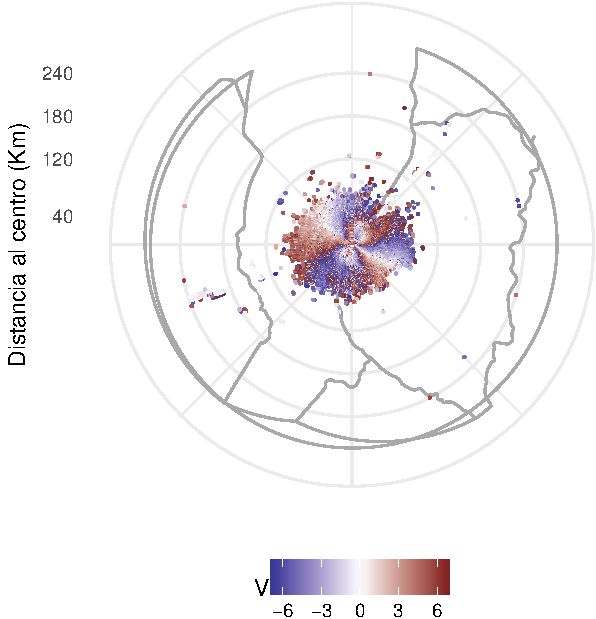
\includegraphics[width=0.48\textwidth, ]{Tesis_files/figure-latex/aliasing-1} }\subfloat[Sin aliasing \label{no-aliasing}\label{fig:aliasing2}]{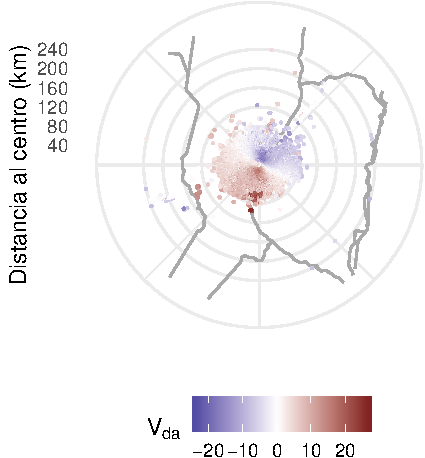
\includegraphics[width=0.48\textwidth, ]{Tesis_files/figure-latex/aliasing-2} }\caption{Velocidad radial (m/s) observada a las 06 UTC por el radar de Paraná en la elevación $1.3^{\circ}$ y $V_N = 6.7 m/s$. Notar las escalas diferentes.}\label{fig:aliasing}
\end{figure}

\section{Velocity Azimuth Display
(VAD)}\label{velocity-azimuth-display-vad}

A medida que el radar rota en la dirección azimutal, mide la velocidad
de los objetivos para cada ángulo y rango de manera continua y en
función del azimut. A esto se le da el nombre de Visualización Azimutal
de la Velocidad o por sus siglas en inglés VAD (por Velocity Azimuth
Display, Lhermitte (1962)) y se muestra en la Figura \ref{vad}. Si el
campo de viento es horizontalmente homogéneo, la velocidad radial media
tiene un comportamiento sinusoidal en función del azimut.

\begin{figure}

{\centering 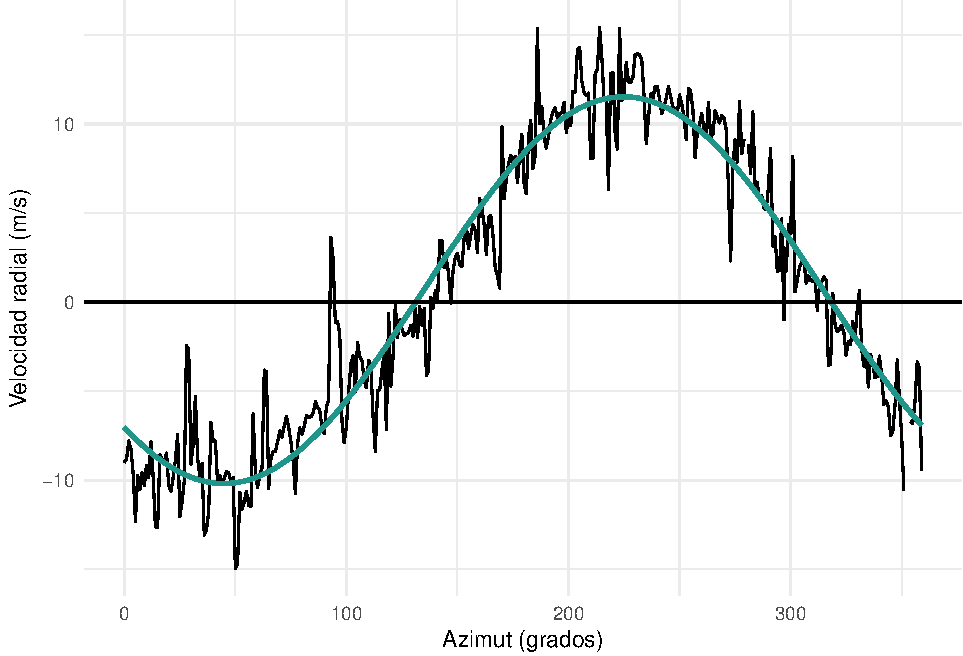
\includegraphics[width=0.75\textwidth]{Tesis_files/figure-latex/vad-1} 

}

\caption{Velocidad radial (m/s) en función del azimut (grados) para un rango y ańgulo de elevación fijos. En color se  ajusta una función sinusoidal a los datos. \label{vad}}\label{fig:vad}
\end{figure}

De esta manera, la velocidad radial medida por el radar corresponde a la
velocidad de un objetivo u obstáculo en el camino del haz. En
situaciones de aire claro (sin nubosidad) es posible tener una medida
del campo de viento dentro de la capa límite usando insectos como
obstáculos. Sin embargo esta velocidad no corresponde al campo de
movimiento real ya que es medida en la dirección radial siendo los
valores negativos movimiento hacia el radar y valores positivos
movimientos desde el radar. Mientras que el valor nulo ocurre en las
regiones donde la velocidad real es perpendicular a la trayectoria del
haz.

A partir de este concepto distintos autores han desarrollado técnicas
para obtener el perfil vertical de viento real a partir del viento
radial o su gradiente con diferentes grados de complejidad. Estas
técnicas son también son llamadas VAD (o sus derivaciones, Browning y
Wexler (1968); Matejka y Srivastava (1991); Gao et~al. (2004); Xu et~al.
(2011)). Para esta tesis se desarrolló un algoritmo para el cálculo del
VAD siguiendo a Browning y Wexler (1968) pero incluyendo controles de
calidad específicos para asegurar la validez de los resultados.

\subsection{Desarrollo matemático}\label{desarrollo-matematico}

El viento radial medido por el radar para un ángulo de elevación
\(\theta\) y rango \(r\) determinado puede expresarse en función del
azimut \(\phi\):

\begin{equation}
\label{eq-vr1}
V_r =  v \cos(\theta) \cos(\phi) + u \cos(\theta) \sin(\phi) - w \sin(\theta)
\end{equation}

Donde \(u\), \(v\) y \(w\) son las componentes del viento en coordenadas
cartesianas.

La Ecuación \ref{eq-vr1} puede ser expresada como suma de una serie de
Fourier de la forma:

\begin{equation}
\label{eq-vr2}
V_r =  \frac{1}{2}a_0 + \sum_{n = 1}^{\infty} (a_n \cos(n\phi) + b_n \sin(n \phi)) 
\end{equation}

Para \(n=1\), los coeficientes de Fourier están asociados al viento en
el centro del dominio de escaneo (con subíndice 0) como:

\begin{equation} \label{eq-vr3}
a_1 = u_0 \cos(\theta) \; y \;
b_1 = v_0 \cos(\theta) 
\end{equation}

A partir de esto es posible ajustar cada anillo de datos de radar, es
decir los datos para cada \(\theta\) y \(r\) realizando una regresión
lineal de la forma:

\begin{equation}
\label{eq-vr4}
V_r \sim a_1\cos \phi + b_1 \sin \phi
\end{equation}

Los coeficientes \(a_0\), \(a_2\) y \(b_2\) no incluidos en el algoritmo
dan información sobre la divergencia horizontal y otras características
del viento, quedando su implementación para futuros trabajos.

Finalmente la velocidad y dirección del viento pueden ser calculadas a
partir de los coeficientes (Ecuaciones \ref{eq-vr3}).

Velocidad:

\begin{equation}
\label{eq-vr5}
V = \frac{(a_{1}^{2} + b_{1}^{2})^{1/2}}{\cos(\theta)}
\end{equation}

Dirección:

\begin{equation}\label{eq-vr6}
\alpha = \frac{\pi}{2}-\tan^{-1}(\frac{a_1}{b_1}) \; \; si \; b_1 < 0 
\end{equation}\begin{equation}\label{eq-vr7}
\alpha = \frac{3\pi}{2}-\tan^{-1}(\frac{a_1}{b_1}) \; \; si \; b_1 > 0
\end{equation}

El resultado de lo anterior un valor de la magnitud del viento y su
dirección para cada anillo asociado a un ángulo de elevación y rango
determinado. Para calcular la altura de cada anillo es necesario conocer
la propagación del haz del radar. La propagación depende del indice de
refracción de la atmósfera (N) y este a su vez de la densidad del aire y
por lo tanto de las condiciones de temperatura y humedad del momento.
Existen distintas metodologías para obtener calcular la propagación del
haz del radar (Zeng et~al., 2014) que varían en su complejidad y
precisión.

En el algoritmo de VAD desarrollado se aplica el modelo 4/3 del radio de
la Tierra. Este modelo es utilizado por la mayoría de los programas de
procesamiento de datos de radar ya que pese a su simpleza (no toma en
cuenta las condiciones de la atmósfera) es aceptable para cualquier
ángulo de elevación usado, alturas máximas de entre 10 y 20 km siempre
que el gradiente de N esté alrededor de \(-1/a\) donde \(a\) es el radio
de la tierra (Doviak y Zrnić, 1993).

Por otro lado se calcula la raíz del error cuadrático medio asociado a
cada anillo (\(rmse_a\)) para estimar la diferencia entre las
observaciones y el modelo estimado:

\begin{equation}\label{eq-vr8}
rmse_a = \sqrt {\sum \frac {(V_r - V_{rmod} )^2} {n-3}}
\end{equation}

donde \(n\) es el número de observaciones presentes en un anillo
particular.

Para obtener un único perfil vertical de viento se interpola un promedio
pesado del valor de las variaciones de los anillos de cada capa de
atmósfera a una grilla vertical equiespaciada preestablecida.

El algoritmo identifica los datos de \(V\) para cualquier rango y ángulo
de elevación que se encuentran en \(z \pm d/2\) donde \(z\) es el punto
de grilla y \(d\) es la resolución espacial de la grilla vertical. Para
obtener el valor promedio de de \(V\) correspondiente a la altura \(z\)
calcula un promedio pesando la variable por el \(rmse_a\) y la distancia
de cada anillo al radar \(r\). De esta manera los anillos con mayor
error y más alejados a punto donde se está estimando la velocidad y
dirección del viento tienen menor influencia en el resultado final.\\

\begin{equation}\label{eq-vr9}
\bar{V} = \frac {\sum w_i V_i} {\sum w_i}
\end{equation}

Donde \(w_i = \frac {1}{rmse_{ai} + r_i}\) y el subíndice \(i\) cuenta
la cantidad de datos para cada intervalo \(z \pm d/2\). De manera
análoga se calcula la dirección del viento para cada punto de grilla
vertical.

Finalmente se calcula el error de estimación asociado a cada punto de
dos maneras:

\begin{itemize}
\tightlist
\item
  \textbf{\(rmse_1\)}
\end{itemize}

\begin{equation}\label{eq-vr10} 
rmse_1 = \frac{\sigma}{\sqrt{n}}
\end{equation}

Donde \(n\) es la cantidad de anillo en esa capa y
\(\sigma^{2}= \frac{\sum (V_i - \bar{V})^2 /rmse_{ai}^2}{\sum 1/rmse_{ai}^2}\)
con \(\bar{V}\) el promedio pesado de la velocidad del viento para la
capa.

Este error relativo da cuenta de la distancia entre el la velocidad
promedio calculada para ese nivel y el valor de cada anillo pesada por
el error del anillo. De esta manera si el \(rmse_{ai}\) es grande la
diferencia \((V_i - \bar{V})^2\) tiene menor peso en el error del nivel.
Por otro lado el denominador suma la inversa de errores de todos los
anillos y por lo tanto mayores errores individuales generan un
\(rmse_1\) mayor. Es importante notar que \(V_i\) y \(\bar{V}\) no están
necesariamente a la misma altura ya que \(\bar{V}\) es el promedio de
muchos \(V_i\) dentro de una capa.

\begin{itemize}
\tightlist
\item
  \textbf{\(rmse_2\)}
\end{itemize}

\begin{equation}\label{eq-vr11}
rmse_2 = \sqrt{\frac{1}{\sum \frac{1}{rmse_{ai}^2}}}
\end{equation}

Este rmse no toma en cuenta la posible dispersión de los valores
individuales de los anillos respecto del valor medio pero retiene el
error cuadrático medio de cada anillo y calcula la raíz del error
cuadrático medio del nivel como la suma de la inversa de los errores
individuales.

\subsection{Controles de calidad de los
datos}\label{controles-de-calidad-de-los-datos}

El algoritmo de VAD desarrollado incluye algunos controles de calidad
para evitar errores asociados a problemas intrínsecos a los datos de
radar.

\subsubsection{Antes del ajusta de los
datos}\label{antes-del-ajusta-de-los-datos}

Permiten determinar cuales son los anillos de datos válidos y eliminar
posibles errores aleatorios.

\begin{itemize}
\tightlist
\item
  \textbf{Ángulos de elevación seleccionados:} La presencia de ecos de
  terreno pueden generar que los campos de velocidad radial para los
  primeros ángulos de elevación sean muy ruidosos y sin coherencia
  espacial. En el otro extremo, los ángulos superiores suelen tener
  pocos datos válidos (es decir, no dato faltante) debido a la escasa
  señal cerca del tope de la capa límite y atmósfera libre en días
  claros. Debido a esto es posible seleccionar el rango de ángulos a ser
  analizados y utilizados en el cálculo del VAD.
\item
  \textbf{Selección del dominio de cálculo:} Otro posibilidad para
  evitar los ecos de terreno es definir un radio mínimo por debajo del
  cual no se incluyen los datos para el cálculo de VAD. En el otro
  extremo, es posible definir un radio máximo para limitar el uso de
  datos muy lejanos al centro del volumen de escaneo. Esto es importante
  para evitar inhomogeneidades en el campo de viento horizontal.
\item
  \textbf{Cantidad de datos por anillo:} el algoritmo cuenta la cantidad
  de datos válidos por anillo y se define un porcentaje de datos
  faltantes respecto del total, por ejemplo 20\%. Si se excede al máximo
  definido el anillo es descartado. De esta manera se evita la
  utilización de anillos donde la señal es muy débil.
\item
  \textbf{Hueco continuo en un anillo:} Además de los datos faltantes
  ubicados de manera aleatoria a lo largo de un anillo, los huecos
  continuos pueden ocurrir debido a la falta de señal en una determinada
  región. De acuerdo a Matejka y Srivastava (1991) esto puede generar
  importantes errores en el resultado final, por lo tanto cuando el
  hueco es mayor a 30° de azimut, el anillo se descarta.
\item
  \textbf{Errores aleatorios:} Los errores aleatorios producto de ruido
  del instrumento pueden ser eliminados utilizando un filtro pasa bajo
  (Gao y Droegemeier, 2004). Este control no elimina anillos pero
  produce un suavizado de los datos.
\end{itemize}

\subsubsection{Luego del ajuste}\label{luego-del-ajuste}

\begin{itemize}
\tightlist
\item
  \textbf{R cuadrado:} El \(r^2\) del modelo ajustado (Ecuación
  \ref{eq-vr4}) permite obtener una medida de de la calidad de ese
  modelo respecto de las observaciones. A partir de la exploración de
  resultados preliminares se observó que la definición de un umbral
  mínimo para el \(r^2\) permite descartar anillos que pese a no tener
  datos faltantes eran erróneos.
\end{itemize}

\subsection{Validación}\label{validacion}

Una manera posible de validar los resultados del VAD es comparando
cualitativa o cuantitativamente el perfil vertical de viento generado
con los datos de un radiosondeo en el mismo momento. Debido a la
inexistencia de sondeos en la región de Paraná se exploró la posibilidad
de utilizar datos del Radar INTA Anguil que se encuentra en la provincia
de La Pampa y radiosondeos de la estación del SMN Santa Rosa Aero
(87623). i bien el radar y la estación meteorológica no están en la
misma ubicación, se encuentran a unos 30 km de distancia y por lo tanto
la estación está dentro del dominio de escaneo del radar. Sin embargo se
encontró que la señal de \(V_r\) en días de cielo claro es muy pobre y
por lo tanto no supera los controles de calidad impuestos en el
algoritmo.

Pero también es posible reconstruir un campo de velocidad radial
sintética interpolando la velocidad medida por la radiosonda utilizando
la grilla del radar utilizando la Ecuación \ref{eq-vr1}. En este proceso
se asume que el campo de viento tridimensional varía linealmente. Este
campo de velocidad radial sintética \(V_{rs}\) puede ser re transformado
a un perfil vertical de viento utilizando el VAD y comparado con el
sondeo original.

Para este segundo método de validación se utilizaron un volumen de datos
del Radar INTA Anguil del 05 de enero de 2016 a las 12 UTC y los datos
del radiosondeo de la estación del SMN Santa Rosa Aero (87623) para la
misma hora. Además, dado que el resultado de la interpolación del viento
real da un campo homogéneo, sin errores o datos faltantes, se aplicaron
distintas fuentes de errores para que la validación sea más realista.

\subsubsection{Pruebas}\label{pruebas}

\begin{itemize}
\tightlist
\item
  \textbf{Sin datos faltantes ni errores (SE)}
\end{itemize}

Se obtiene el \(V_r\) interpolado a la grilla del radar de Anguil (con
una estrategia de escaneo hasta 120 km de radio y 8 ángulos de
elevación) a partir del sondeo. Como los datos de sondeo llegan hasta
los 30 km de altura, hay información disponible para interpolar los
datos de \(V-r\) para todos los ángulos de elevación y para cualquier
rango. Sin embargo esto nos da muchos más datos de los disponibles
normalmente. Es de esperar que el VAD resultante sea muy similar al
sondeo y inicial pero esta primera validación también permite verificar
que la transformación de \(V\) a \(V_r\) es correcta.

\begin{figure}
\subfloat[Datos de radar \label{radar}\label{fig:validacion1}]{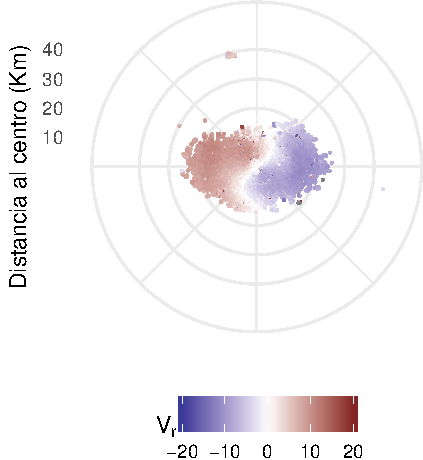
\includegraphics[width=0.48\textwidth, ]{Tesis_files/figure-latex/validacion-1} }\subfloat[Sin errores \label{se}\label{fig:validacion2}]{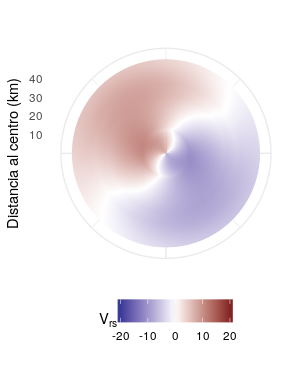
\includegraphics[width=0.48\textwidth, ]{Tesis_files/figure-latex/validacion-2} }\newline\subfloat[Con errores \label{ce}\label{fig:validacion3}]{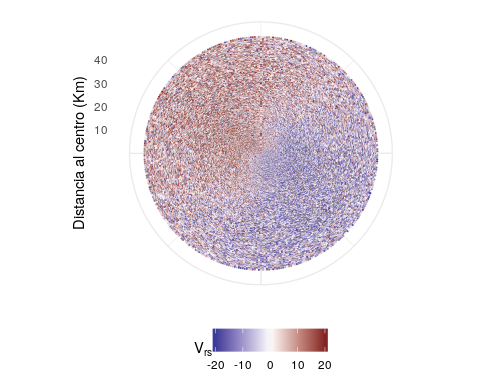
\includegraphics[width=0.48\textwidth, ]{Tesis_files/figure-latex/validacion-3} }\subfloat[Con errores + NAs \label{na}\label{fig:validacion4}]{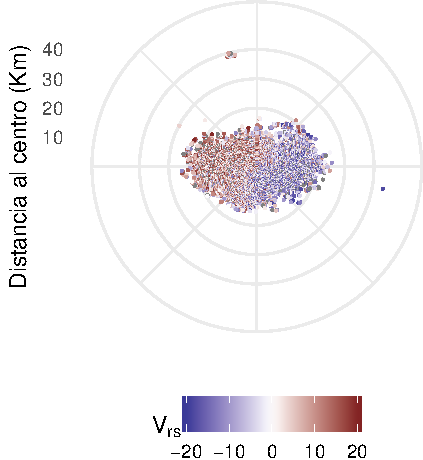
\includegraphics[width=0.48\textwidth, ]{Tesis_files/figure-latex/validacion-4} }\caption{Velocidad radial (m/s) observada a las 12 UTC por el radar de Anguil en la elevación $1.3^{\circ}$ y la misma variable transformada a partir del sondeo de la estación Santa Rosa Aero para la misma hora \label{validacion}}\label{fig:validacion}
\end{figure}

En la Figura \ref{validacion} se puede observar el campo de \(V_r\)
observado por el radar (izquierda) y el campo de \(V_{rs}\) obtenidos a
partir del sondeo. Cualitativamente se observa que tanto la magnitud
como la dirección del viento son similares pero también que el \(V_rs\)
cubre totalmente el dominio mientras que la señal del \(V_r\) se
extingue a los 15 km de rango. Cuantitativamente la diferencia
\(V_r - V_{rs}\) es grande en puntos localizados pero la media absoluta
es de 2.08 m/s, un valor razonable teniendo en cuenta que las
observaciones son realizadas por instrumentos distintos.

\begin{itemize}
\tightlist
\item
  \textbf{Con errores aleatorios (EA)}
\end{itemize}

Para realizar una validación más realista se agregaron errores
aleatorios al campo de \(V_{rs}\), esto además permite analizar la
sensibilidad del algoritmo a este tipo de errores.

El nuevo campo perturbado será:

\begin{equation} \label{eq-vr12}
V_{rs}'  = V_{rs} + \alpha \varepsilon(0,1)
\end{equation}

Donde \(\alpha\) es la amplitud del error y \(\varepsilon\) es un número
aleatorio con distribución normal, \(\mu = 0\) y \(\sigma= 1\).

En la Figura \ref{ce} se muestra el campo resultante utilizando
\(\alpha = 1 m/s\), rápidamente se ve la variabilidad impuesta y también
la disminución en la coherencia horizontal aunque se mantiene
aproximadamente el signo de la variable en las distintas regiones.

\begin{itemize}
\tightlist
\item
  \textbf{Con errores aleatorios y datos faltantes (EA+NA)}
\end{itemize}

Otro problema importante en los datos de radar es la ausencia de señal,
esto se ve como datos faltantes (NAs). Para analizar el efecto de los
datos faltantes se aplicó una máscara de NAs al campo de \(V_{rs}'\) de
tal manera que sean los mismo NAs presentes en el volumen de datos de
radar utilizados (Figura \ref{na}).

\subsubsection{Perfiles obtenidos}\label{perfiles-obtenidos}

En la Figura \ref{validacion-perfiles} se muestra el perfil del sondeo
para los primeros 3 km de altura y los perfiles calculado con VAD a
partir de los distintos campos sintéticos. En cuanto a la magnitud no se
ven diferencias importantes y al observar el detalle de los primeros
1000 metros de altura, la diferencia es menor a 0.5 m/s en todos los
casos. Tampoco se observó sensibilidad al aumento de la amplitud de
error (no se muestra).

\begin{figure}
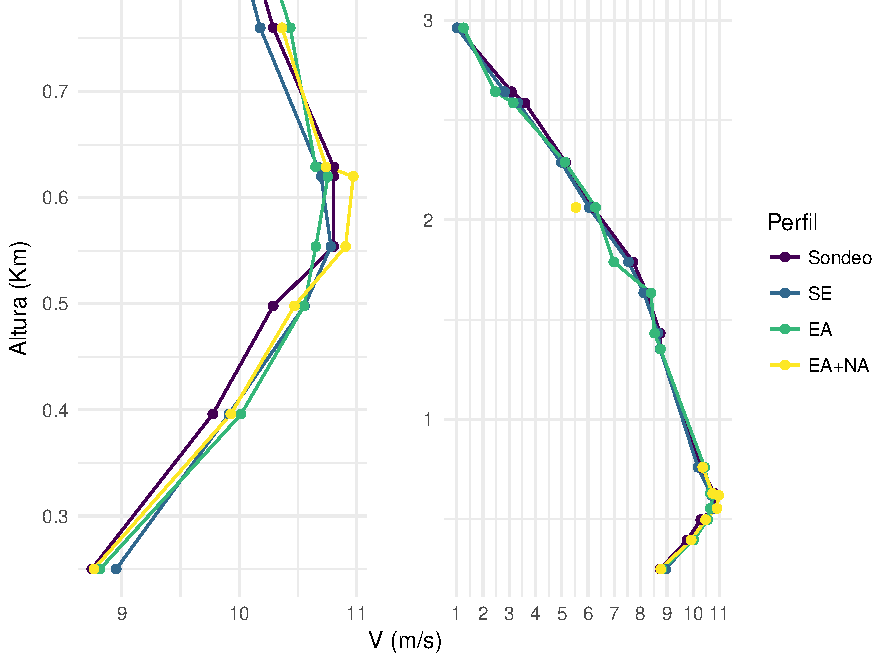
\includegraphics[width=0.95\textwidth, ]{Tesis_files/figure-latex/validacion-perfiles-1} \caption{Viento medio (m/s) en función de la altura a partir del sondeo, y las distintas pruevas de validación a la izquierda y el detalle ampliado del máximo en niveles bajos \label{validacion-perfiles}}\label{fig:validacion-perfiles}
\end{figure}

Esto puede verificarse con el cálculo de distintos errores (Gao y
Droegemeier, 2004): la raíz del error cuadrático medio
(\(rms = \sqrt{ \frac{\sum (V-V_{ref})^2}{N} }\)) y el error relativo al
rms (\(rre = \sqrt{ \frac{\sum (V-V_{ref})^2}{\sum (V_{ref})^2} }\))
donde \(V_{ref}\) corresponde a la variable de referencia, en este caso
el sondeo. Los resultados se muestran en la Tabla
\ref{validacion-errores} y como puede observarse no hay un aumento
importante al incorporar errores aleatorios y disminuye al quitar datos
en la prueba EA+NA ya que los errores calculados son sensibles a la
cantidad total de datos.

\begin{longtable}[]{@{}lrr@{}}
\caption{Errores calculados para las distintas pruebas de
validación.}\tabularnewline
\toprule
Prueba & rms & rre\tabularnewline
\midrule
\endfirsthead
\toprule
Prueba & rms & rre\tabularnewline
\midrule
\endhead
SE & 0.1613 & 0.0194\tabularnewline
EA & 0.3020 & 0.0364\tabularnewline
EA+NA & 0.1778 & 0.0214\tabularnewline
\bottomrule
\end{longtable}

El efecto más importante en las pruebas de validación corresponde a la
presencia de NAs. La falta de datos en distintas regiones para rangos a
partir de 10 a 15 km impide el cálculo del perfil por encima de 800
metros (con excepción de un punto a los 2000 metros de altura).

\section{Consistencia temporal de las
observaciones}\label{consistencia-temporal-de-las-observaciones}

Ya que uno de los objetivos de esta tesis es estudiar la evolución del
viento a lo largo del día, es importante asegurar cierta consistencia
temporal en los datos. La inconsistencia temporal puede deberse a que
cada volumen de datos no es medido de manera instantánea si no que
demora algunos minutos. Si bien en periodos sin cambios sinópticos
importantes no se espera variaciones bruscas del viento, es posible que
variaciones menores a los 10 minutos (resolución temporal de los datos
de radar) estén afectando la consistencia temporal.

Para solucionar este problema se aplicó un suavizado pesado localmente o
LOWESS (locally weighted scatterplot smoothing, Cleveland (1979)).
LOWESS es un método de regresión no paramétrica y por lo tanto no es
necesario asumir que los datos tienen algún tipo de distribución
particular. Esto lo hace un método flexible al representar el
comportamiento de los datos. Por otro lado la estimación para cada punto
se realiza utilizando la información de datos vecinos. Para esto se
especifica cuantos datos vecinos se utilizaran para estimar cada punto
local como una fracción del total de datos.

Aplicación de este método permite eliminar variaciones temporales
bruscas entre sets de datos y mejorar la coherencia.

\textbf{Necesito mostrar como quedan los datos acá? No quiero spoilear
los resultados}

\section{Tratamiento de procesos en la
CLP}\label{tratamiento-de-procesos-en-la-clp}

El estudio de los procesos que ocurren en la CLP es un desafío cuando no
se cuentan con datos de la turbulencia. En esta tesis se abordan
procesos que pueden ser estudiados a partir de los perfiles de viento y
las variables de superficie.

\subsection{Determinación del estado de la
turbulencia}\label{determinacion-del-estado-de-la-turbulencia}

El número de Richarson puede ser utilizado como un estimador de la
estabilidad dinámica (Stull, 1988) y por lo tanto de la turbulencia
presente. A partir de algunas suposiciones como la valides de la teoría
K es posible escribir el número de Richarson en termino de gradientes:

\begin{equation} \label{eq-ri1}
R_i = \frac{\frac{g}{\overline{\theta_v}} \frac{\partial \overline{\theta_v}}{\partial z}}
{\left [ \left (\frac{\partial \overline{u}}{\partial z} \right )^2 + \left (\frac{\partial \overline{v}}{\partial z} \right )^2  \right]}
\end{equation}

El numerador de la Ecuación \ref{eq-ri1} da cuenta de los procesos
boyantes que tienen a destruir la turbulencia en condiciones estables y
a producirla en condiciones inestables. El denominador corresponde a la
producción mecánica o por cortante. De acuerdo a Stull (1988) la
turbulencia puede mantenerse si \(R_i < R_T\), ya que por encima de este
umbral (en general \(R_T = 1\)), el flujo turbulento se vuelve laminar.

Debido a que la estimación de los gradientes suele ser difícil, estos
suelen ser expresados en términos de observaciones discretas. Surge así
el número de Richarson Bulk:

\begin{equation} \label{eq-ri2}
R_b = \frac{g \, \Delta \overline{\theta_v} \, \Delta z}{\overline{\theta_v} \, [(\Delta \overline{u}^2) + [(\Delta \overline{v}^2)]}
\end{equation}

Para obtener el \(R_b\) en cada tiempo y su variación con la altura es
necesario, entonces con el perfil vertical de temperatura virtual
(\(\theta_v\)), y de la velocidad del viento. Debido a que solo se
cuenta con el valor de la temperatura en superficie, se utilizó la
siguiente aproximación válida para estimar el número de Richarson en el
periodo estable:

\begin{equation} \label{eq-ri3}
R_i \sim \frac{(g  \: (\theta_i - \theta_f)/z_{máx})}{(\overline{\theta} \: (u_{máx}/z_{máx})^2)}
\end{equation}

Donde \(\theta_i\) corresponde al valor de la temperatura virtual en
superficie en el momento de transición entre la capa mezclada y el
comienzo de la capa estable nocturna, por lo tanto será la temperatura
en el tope de la capa estable asumiendo que la capa residual no se
modifica. El valor de \(\theta_f\) será la temperatura en superficie
observado. Por último \(u_{máx}\) es el valor máximo de viento observado
y \(z_{máx}\), la altura a la que ocurre este máximo y que coincide con
el tope de la capa estable (Ver Sección \ref{sec-pbh}).

\subsection{\texorpdfstring{Altura de la capa límite
\label{sec-pbh}}{Altura de la capa límite }}\label{altura-de-la-capa-limite}

La altura de la capa límite se define como la altura a la cual las
características de la superficie no afecta la atmósfera. Las
estimaciones de esta variable son muy diversas en la literatura y
también sus aplicaciones a los modelos numéricos.

Por ejemplo la altura de la capa estable nocturna puede definirse como
la altura a la cual la intensidad de la turbulencia es una fracción del
valor en superficie mientras que la altura de la capa mezclada puede
determinarse como la altura a la que se observa el menor transporte
vertical de calor.

Teniendo en cuenta los datos disponibles se determinará la altura de la
capa estable nocturna como la altura a la que ocurre el máximo de
viento.

\textbf{Ver si resulta lo de usar dBZ o si se puede hacer algo con la
altura de la capa mezclada}

\subsection{Detección del LLJ}\label{deteccion-del-llj}

El Jet nocturno de capas cajas o LLJ (Low Level Jet) es un fenómeno de
mesoescala caracterizado por por una corriente fuerte de viento con
máximos de entre 10 y 20 m/s que se localiza en los primeros cientos de
metros de altura (Stull, 1988). Su extensión vertical es poca pero
horizontalmente puede extenderse por cientos de kilómetros. De acuerdo a
Vera et~al. (2006) en la región de Paraná el LLJ es observado
frecuentemente en la estación de verano entre las 00 y las 06 UTC.

Existen distintos criterios para identificar el LLJ, en algunos casos se
determina un umbral mínimo para la velocidad del viento a partir del
cual se considera la existencia del LLJ siempre que este ocurra por
debajo de algún nivel determinado. En otros casos, se busca que el
viento sea supergeostrófico. En este trabajo se utilizará el criterio de
Bonner (1968) que identifica el LLJ cuando el máximo del viento es
superior a 12 m/s y decrece al menos 6 m/s hasta el próximo mínimo o
hasta el nivel de 3 km.

El LLJ puede producirse por distintos mecanismos entre los que se pueden
nombrar la topografía, baroclinicidad asociada a pendientes del terreno,
frentes y oscilaciones inerciales. En algunas situaciones, varios
mecanismos pueden contribuir a la formación del LLJ de manera conjunta.

De acuerdo a Blackadar (1957) luego del atardecer, cuando no hay
producción de turbulencia se produce un desacople de la capa mezclada y
el viento tiende a acelerarse ante la ausencia de la fricción hacia el
equilibrio geostrófico. Sin embargo la fuerza de Coriolis genera una
oscilación inercial del viento alrededor del viento geostrófico
produciendo un LLJ supergeostrófico durante el periodo estable.

Esta oscilación puede verse en la rotación del vector del viento con la
altura (hodógrafa), que para el hemisferio sur será en sentido
antihorario. El periodo de la oscilación inercial es de \(P = 2\pi/f\),
con \(f\) el parámetro de Coriolis. A la latitud de Paraná \(P = 17.79\)
horas y por lo tanto se espera que el máximo viento ocurra para cuando
se alcanza la mitad del periodo desde el atardecer (Kallistratova y
Kouznetsov, 2012).

\section{WRF}\label{wrf}

\begin{figure}

{\centering \subfloat[Dominio utilizado en el modelo con resolución de 12 km (dominio exterior) y 4 km (dominio interior. El punto representa la ubicación del radar. \label{dom-modelo}\label{fig:dominio1}]{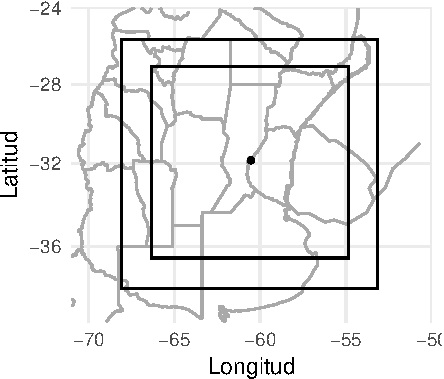
\includegraphics[width=0.48\textwidth]{Tesis_files/figure-latex/dominio-1} }\hfill\subfloat[Topografía sobre el nivel del radar. El circulo negro coresponde al dominio de análisis, de 40km de radio y centrado en el radar. \label{dom-radar}\label{fig:dominio2}]{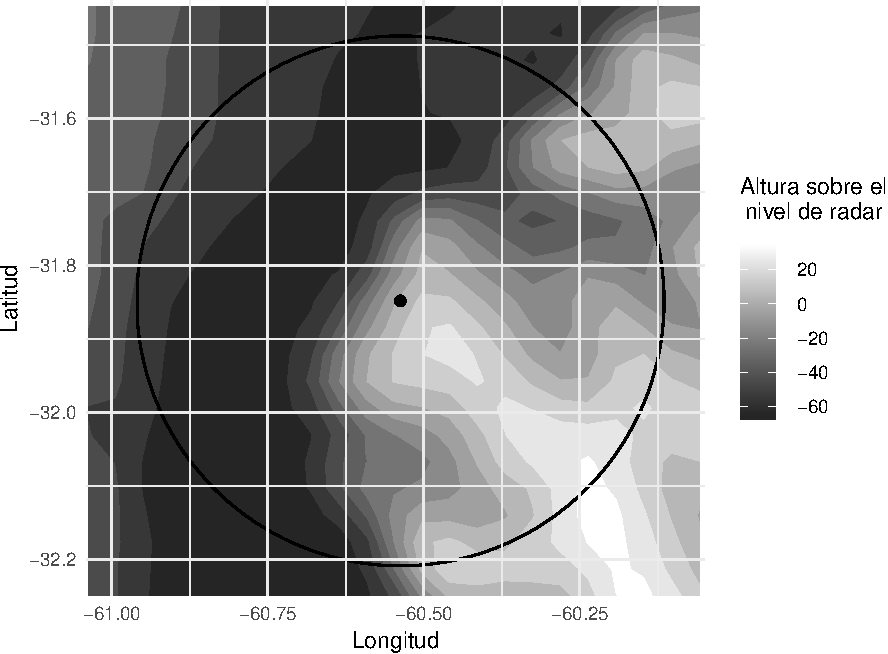
\includegraphics[width=0.48\textwidth]{Tesis_files/figure-latex/dominio-2} }

}

\caption{Dominios utilizados. \label{dominio}}\label{fig:dominio}
\end{figure}

Presentación de la idea: sensibilidad del esquema de PBL Dominio Periodo
modelado Niveles verticales utilizados debido al efecto sobre la altura
de la capa límite. Parametrizaciones usadas (no PBL)

\subsection{Parametrizaciones}\label{parametrizaciones}

Características principales de las parametrizaciones usadas.

\chapter{Resultados}\label{resultados}

\section{Análisis descriptivo de los
casos}\label{analisis-descriptivo-de-los-casos}

\subsection{caracteristicas generales y
sinopticas}\label{caracteristicas-generales-y-sinopticas}

\section{Análisis de los VAD
obtenidos}\label{analisis-de-los-vad-obtenidos}

\section{Análisis de la turbulencia}\label{analisis-de-la-turbulencia}

\section{Análisis cualitativo de la oscilación
inercial}\label{analisis-cualitativo-de-la-oscilacion-inercial}

\section{Analisis de las corridas y comparación con
obs}\label{analisis-de-las-corridas-y-comparacion-con-obs}

\chapter{Conclusiones}\label{conclusiones}

\chapter*{Referencias}\label{referencias}
\addcontentsline{toc}{chapter}{Referencias}

\hypertarget{refs}{}
\hypertarget{ref-Acevedo2014}{}
Acevedo, O.C., Costa, F.D., Oliveira, P.E.S., Puhales, F.S., Degrazia,
G.A., y Roberti, D.R., 2014. The Influence of Submeso Processes on
Stable Boundary Layer Similarity Relationships. Journal of the
Atmospheric Sciences, 71, 1, 207-225.

\hypertarget{ref-Banks2016}{}
Banks, R.F., Tiana-Alsina, J., Baldasano, J.M., Rocadenbosch, F.,
Papayannis, A., Solomos, S., y Tzanis, C.G., 2016. Sensitivity of
boundary-layer variables to PBL schemes in the WRF model based on
surface meteorological observations, lidar, and radiosondes during the
HygrA-CD campaign. Atmospheric Research, 176-177, 185-201.

\hypertarget{ref-Berri2012}{}
Berri, G.J., Nuin, J.S.G., Sraibman, L., y Bertossa, G., 2012.
Verification of a Synthesized Method for the Calculation of Low-Level
Climatological Wind Fields Using a Mesoscale Boundary-Layer Model.
Boundary-Layer Meteorology, 142, 2, 329-337.

\hypertarget{ref-Blackadar1957}{}
Blackadar, A.K., 1957. Boundary Layer Wind Maxima and Their Significance
for the Growth of Nocturnal Inversions. Bulletin of the American
Meteorological Society, 38, 5, 283-290.

\hypertarget{ref-Bonner1968}{}
Bonner, W.D., 1968. Climatology of the Low Level Jet. Monthly Weather
Review, 96, 12, 833-850.

\hypertarget{ref-Bousquet2008}{}
Bousquet, O., Montmerle, T., y Tabary, P., 2008. Using operationally
synthesized multiple-Doppler winds for high resolution horizontal wind
forecast verification. Geophysical Research Letters, 35, 10, 1-6.

\hypertarget{ref-Browning1968}{}
Browning, K.A., y Wexler, R., 1968. The Determination of Kinematic
Properties of a Wind Field Using Doppler Radar.

\hypertarget{ref-Cleveland1979}{}
Cleveland, W.S., 1979. Robust Locally Weighted Regression and Smoothing
Scatterplots. Journal of the American Statistical Association, 74, 368,
829-836.

\hypertarget{ref-Doviak1993}{}
Doviak, R.J., y Zrnić, D.S., 1993. Doppler Radar and Weather
Observations, Segunda Ed., Academic Press, Inc., Vol. 33, p. 545.

\hypertarget{ref-Gao2004}{}
Gao, J., y Droegemeier, K., 2004. A variational technique for dealiasing
Doppler radial velocity data. Journal of Applied Meteorology, 43, 1990,
934-940.

\hypertarget{ref-Gao2004a}{}
Gao, J., Droegemeier, K.K., Gong, J., y Xu, Q., 2004. A Method for
Retrieving Mean Horizontal Wind Profiles from Single-Doppler Radar
Observations Contaminated by Aliasing. Monthly Weather Review, 132,
1982, 1399.

\hypertarget{ref-Gassmann2001}{}
Gassmann, M.I., y Mazzeo, N.A., 2001. Nocturnal stable boundary layer
height model and its applications. Atmospheric Research, 47, 159-247.

\hypertarget{ref-Haase2004}{}
Haase, G., y Landelius, T., 2004. Dealiasing of Doppler radar velocities
using a torus mapping. Journal of Atmospheric and Oceanic Technology,
21, 10, 1566-1573.

\hypertarget{ref-Helmus2016}{}
Helmus, J.J., y Collis, S.M., 2016. The Python ARM Radar Toolkit (
Py-ART ), a Library for Working with Weather Radar Data in the Python
Programming Language. Journal of Open Research Software, 4, 1, e25.

\hypertarget{ref-Holleman2008}{}
Holleman, I., Gasteren, H. van, y Bouten, W., 2008. Quality assessment
of weather radar wind profiles during bird migration. Journal of
Atmospheric and Oceanic Technology, 25, 12, 2188-2198.

\hypertarget{ref-Kallistratova2012}{}
Kallistratova, M.A., y Kouznetsov, R.D., 2012. Low-Level Jets in the
Moscow Region in Summer and Winter Observed with a Sodar Network.
Boundary-Layer Meteorology, 143, 1, 159-175.

\hypertarget{ref-Lhermitte1962}{}
Lhermitte, R.M., 1962. Note on Wind Variability with Doppler Radar.
Journal of the Atmospheric Sciences, 19, 343-346.

\hypertarget{ref-Lim2010}{}
Lim, E., y Sun, J., 2010. A Velocity dealiasing technique using rapidly
updated analysis from a four-dimensional variational doppler radar data
assimilation system. Journal of Atmospheric and Oceanic Technology, 27,
7, 1140-1152.

\hypertarget{ref-Matejka1991}{}
Matejka, T., y Srivastava, R.C., 1991. An Improved Version of the
Extended Velocity Azimuthh Display Analysis of Single-Doppler Radar
Data. Journal of Atmospheric and Oceanic Technology, 8, 4, 453-466.

\hypertarget{ref-Mazzeo1990}{}
Mazzeo, N.A., y Gassmann, M.I., 1990. Mixing heights and wind direction
analysis for urban and suburban areas of Buenos Aires city. Energy and
Buildings, 15, 3-4, 333-337.

\hypertarget{ref-Rennie2010}{}
Rennie, S.J., Illingworth, A.J., Dance, S.L., y Ballard, S.P., 2010. The
accuracy of Doppler radar wind retrievals using insects as targets.
Meteorological Applications, 17, 4, 419-432.

\hypertarget{ref-Rennie2011}{}
Rennie, S.J., Dance, S.L., Illingworth, A.J., Ballard, S.P., y Simonin,
D., 2011. 3D-Var assimilation of insect-derived Doppler radar radial
winds in convective cases using a high resolution model.
\(\backslash\)Mwr, 139, 4, 1148-1163.

\hypertarget{ref-Rizza2013}{}
Rizza, U., Miglietta, M.M., Acevedo, O.C., Anabor, V., Degrazia, G.A.,
Goulart, A.G., y Zimmerman, H.R., 2013. Large-eddy simulation of the
planetary boundary layer under baroclinic conditions during daytime and
sunset turbulence. Meteorological Applications, 20, 1, 56-71.

\hypertarget{ref-Ruiz2010}{}
Ruiz, J.J., Saulo, C., y Nogués-Paegle, J., 2010. WRF Model Sensitivity
to Choice of Parameterization over South America: Validation against
Surface Variables. Monthly Weather Review, 138, 8, 3342-3355.

\hypertarget{ref-Ruiz2015}{}
Ruiz, J.J., Miyoshi, T., Satoh, S., y Ushio, T., 2015. A Quality Control
Algorithm for the Osaka Phased Array Weather Radar. Sola, 11, 0, 48-52.

\hypertarget{ref-Saibene2014}{}
Saibene, Y.B., Banchero, S., y Pampa, L., 2014. Desarrollo y uso de
herramientas libres para la explotación de datos de los radares
meteorológicos del INTA. En pp. 74-86.

\hypertarget{ref-Salonen2008}{}
Salonen, K., Järvinen, H., Järvenoja, S., Niemelä, S., y Eresmaa, R.,
2008. Doppler radar radial wind data in NWP model validation.
Meteorological Applications, 15, 97-102.

\hypertarget{ref-Skamarock2008}{}
Skamarock, W., Klemp, J., Dudhi, J., Gill, D., Barker, D., Duda, M.,
Huang, X.-Y., Wang, W., y Powers, J., 2008. A Description of the
Advanced Research WRF Version 3.

\hypertarget{ref-Stull1988}{}
Stull, R.B., 1988. An Introduction to Boundary Layer Meteorology,
Primera Ed., Kluwer Academic Publishers, p. 670.

\hypertarget{ref-Tonti2015}{}
Tonti, N.E., y Gassmann, M.I., 2015. Variabilidad del parámetro de
rugosidad sobre una cobertura vegetal. Meteorologica, 40, 2, 59-72.

\hypertarget{ref-Ulke2000}{}
Ulke, A.G., 2000. New turbulent parameterization for a dispersion model
in the atmospheric boundary layer. Atmospheric Environment, 34, 7,
1029-1042.

\hypertarget{ref-Ulke2001}{}
Ulke, A.G., y Andrade, M.F., 2001. Modeling urban air pollution in Sao
Paulo, Brazil: Sensitivity of model predicted concentrations to
different turbulence parameterizations. Atmospheric Environment, 35, 10,
1747-1763.

\hypertarget{ref-Vera2006}{}
Vera, C., Baez, J., Douglas, M., Emmanuel, C.B., Marengo, J., Meitin,
J., Nicolini, M., Nogues-Paegle, J., Paegle, J., y Penalba, O. y otros,
2006. The South American low-level jet experiment. Bulletin of the
American Meteorological Society, 87, 1, 63-77.

\hypertarget{ref-Wang2004}{}
Wang, Y., Xie, S.-P., Xu, H., y Wang, B., 2004. Regional Model
Simulations of Marine Boundary Layer Clouds over the Southeast Pacific
off South America. Part I: Control Experiment*. Monthly Weather Review,
132, 1, 274-296.

\hypertarget{ref-Xie2012}{}
Xie, B., Fung, J.C.H., Chan, A., y Lau, A., 2012. Evaluation of nonlocal
and local planetary boundary layer schemes in the WRF model. Journal of
Geophysical Research Atmospheres, 117, 12, 1-26.

\hypertarget{ref-Xu2011}{}
Xu, Q., Nai, K., Wei, L., Zhang, P., Liu, S., y Parrish, D., 2011. A
VAD-based dealiasing method for radar velocity data quality control.
Journal of Atmospheric and Oceanic Technology, 28, 1, 50-62.

\hypertarget{ref-Zeng2014}{}
Zeng, Y., Blahak, U., Neuper, M., y Jerger, D., 2014. Radar beam tracing
methods based on atmospheric refractive index. Journal of Atmospheric
and Oceanic Technology, 31, 12, 2650-2670.


\end{document}
